\section{Results}
\label{sec:accumulator-results}


The benchmark was ran on \gls{hw1} machine where the client and server parts were distributed in three different ways, namely: within a socket, in two separate sockets of a node and in two separate nodes. Nodes of \gls{hw1} machine are connected via \textit{infiniband} interconnect with the characteristics shown in figure \ref{fig:hw1-bandwidth}. In order to estimate the affect of pure data accumulation, the benchmark, listing \ref{lst:bench:auxiliary-subroutines}, was modified to use only blocking \gls{mpi} operations i.e. \gls{mpi}\_Bcast. We denote the main benchmark as \textbf{BM1} and the modified one as \textbf{BM2} to distinguish and separately explain effects of pure data accumulation and non-blocking data transfer.\\


Figure \ref{fig:benchmark:results-cube-64} represents results of the benchmarks obtained using \textit{cube-64} communication pattern. The client and server parts of the code were distributed in different sockets within the same node. The factor value was chosen to be equal to 1.\\


\begin{figure}[htpb]
\centering
	\begin{tabular}{c}
		\subfloat[communication pattern of \textit{cube-64} \label{fig:benchmark:results-comm-pattern}]{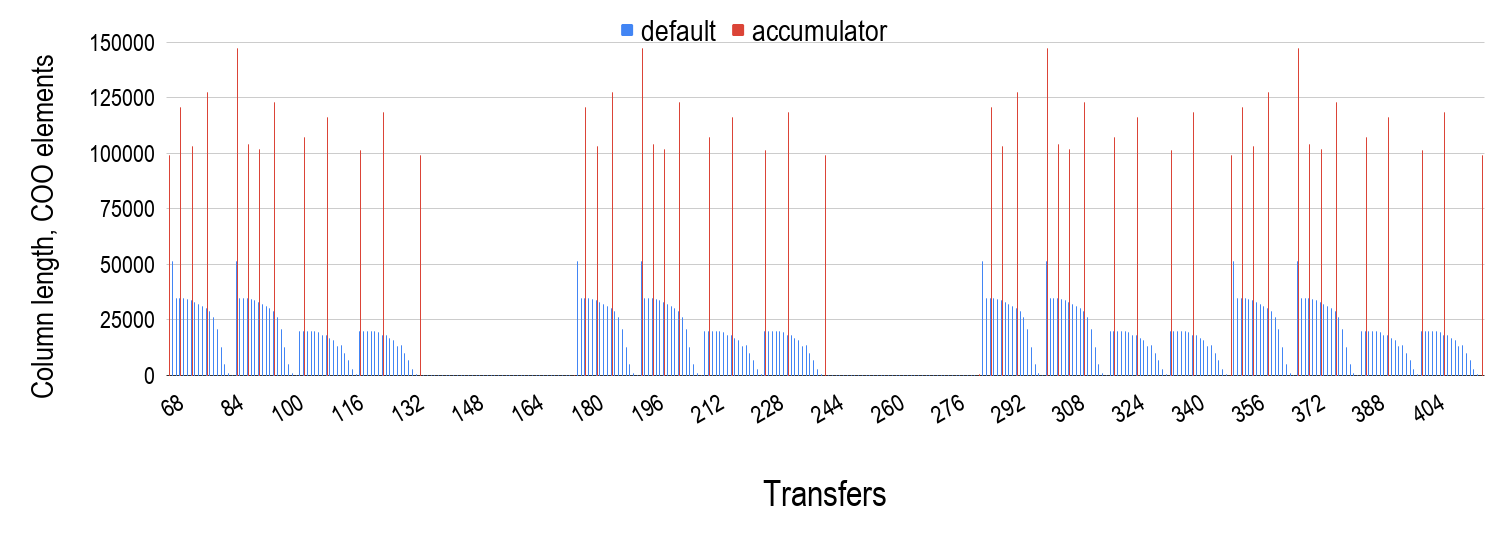
\includegraphics[width=1.0\textwidth]{figures/chapter-3/benchmark-communication-pattern.png}} \\
		\subfloat[BM2: comparison of data accumulation and blocking communication with the default approach]{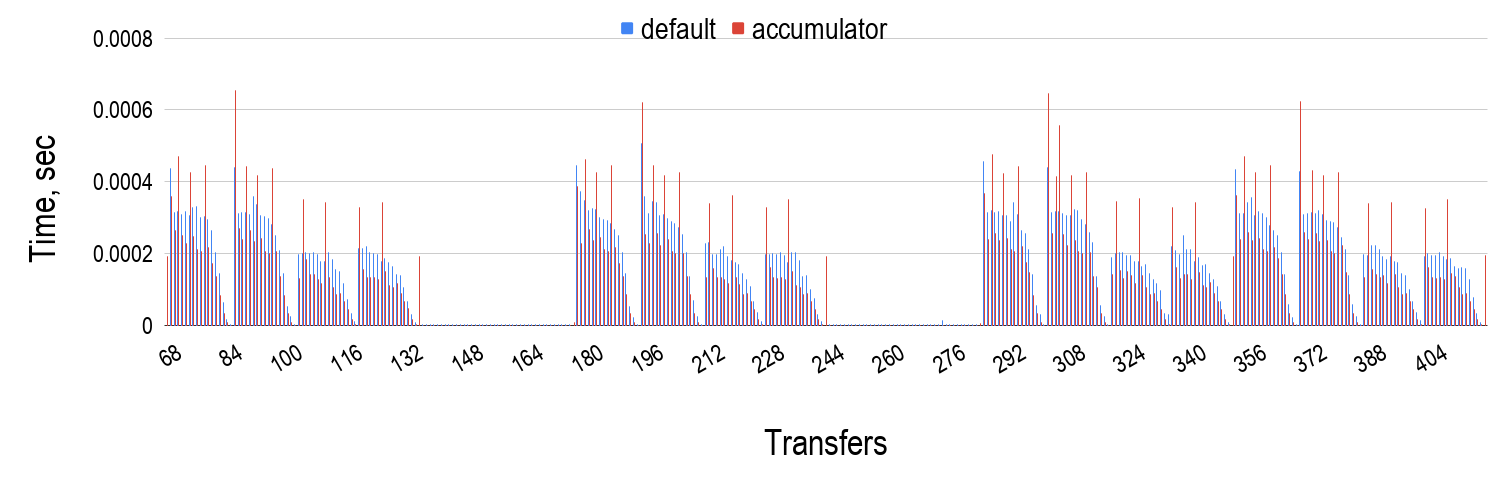
\includegraphics[width=1.0\textwidth]{figures/chapter-3/benchmark-result-blocking.png}} \\
		\subfloat[BM1: comparison of data accumulation and non-blocking communication with the default approach]{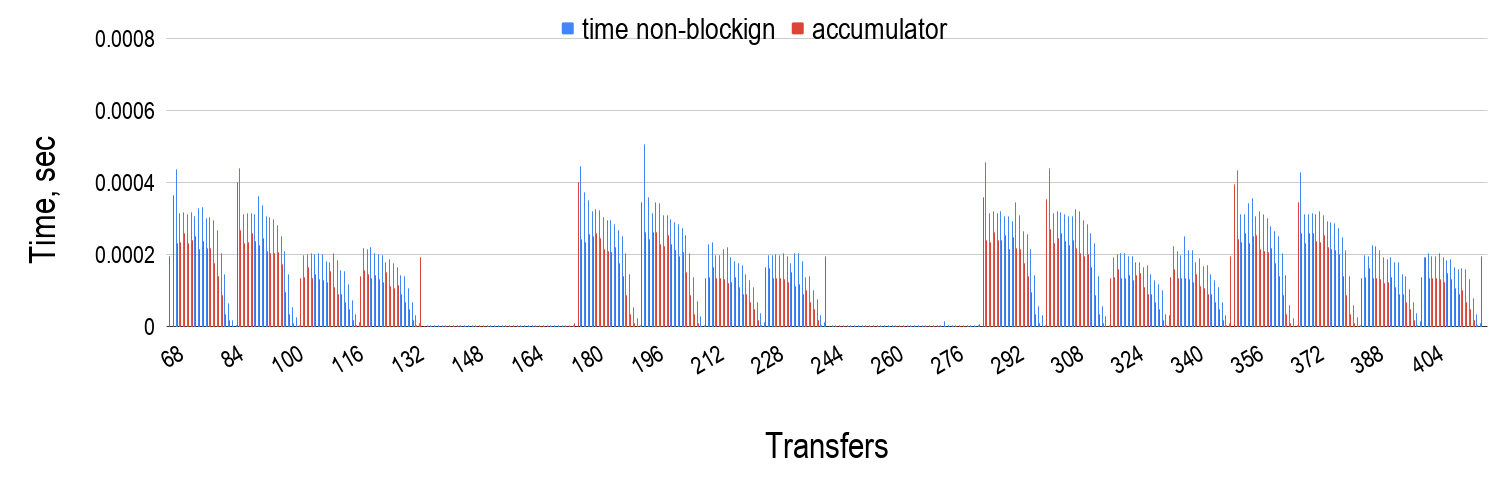
\includegraphics[width=1.0\textwidth]{figures/chapter-3/benchmark-result-non-blocking.png}}
	\end{tabular}
	\caption{Comparison of benchmarks running recorded \textit{cube-64} communication pattern between two sockets within a node}
	\label{fig:benchmark:results-cube-64}
\end{figure}


Figure \ref{fig:benchmark:results-comm-pattern} shows that \textit{accumulator} approach resulted in more that \textbf{6} times drop, from \textbf{344} to \textbf{51}, of the total number of data transfers and resulting resource acquisitions, within the range depicted on the graphs. According to \textbf{BM2} benchmark, the accumulation effect allowed to reduce the run-time by almost \textbf{9\%} by means of more efficient utilization of intra-node interconnection. The obtained results  also demonstrated that overall effect of both accumulation and non-blocking data transfer decreased the run-time of \textbf{BM1} benchmark in more than \textbf{26\%}. Table \ref{table:benchmark:performance-gain} summarizes results obtained for all three client-server distributions within the same range of the recorded communication pattern displayed in figure \ref{table:benchmark:performance-gain}.\\


\begin{table}[ht]
\centering
\begin{tabular}{|c|c|c|}
\hline
\begin{tabular}[c]{@{}c@{}}Benchmark\\ name\end{tabular} & BM2, \% & BM1, \% \\ \hline
within a socket                                          & 7.61    & 13.84   \\ \hline
between sockets                                          & 9.04    & 26.26   \\ \hline
between nodes                                            & -2.06   & 3.20    \\ \hline
\end{tabular}
\caption{Time reduction in contrast to the default approach in case of \textit{cube-64} communication pattern}
\label{table:benchmark:performance-gain}
\end{table}


It turned out that \textbf{BM2} benchmark was slower than the default \gls{athlet} approach in  approximately \textbf{2\%} in case of the inter-node communication. However, non-blocking data broadcast, according to \textbf{BM1} benchmark, helped to alleviate the slow-down and achieve almost \textbf{3\%} of improvement.\\


Unimpressive results of non-blocking the inter-node communication can be explained by specifics of the benchmark design. In particular, time spent on generation of random matrix elements was not enough to overlap time spent on non-blocking data transfer in case of \textit{cube-64} test case, see figure \ref{fig:benchmark:results-cube-64-inter-node-comm}. Hence, the execution control was probably suspended by \gls{mpi} library at the subsequent call of \textit{MPI\_Wait()} function.\\


\begin{figure}[htpb]
  \centering
  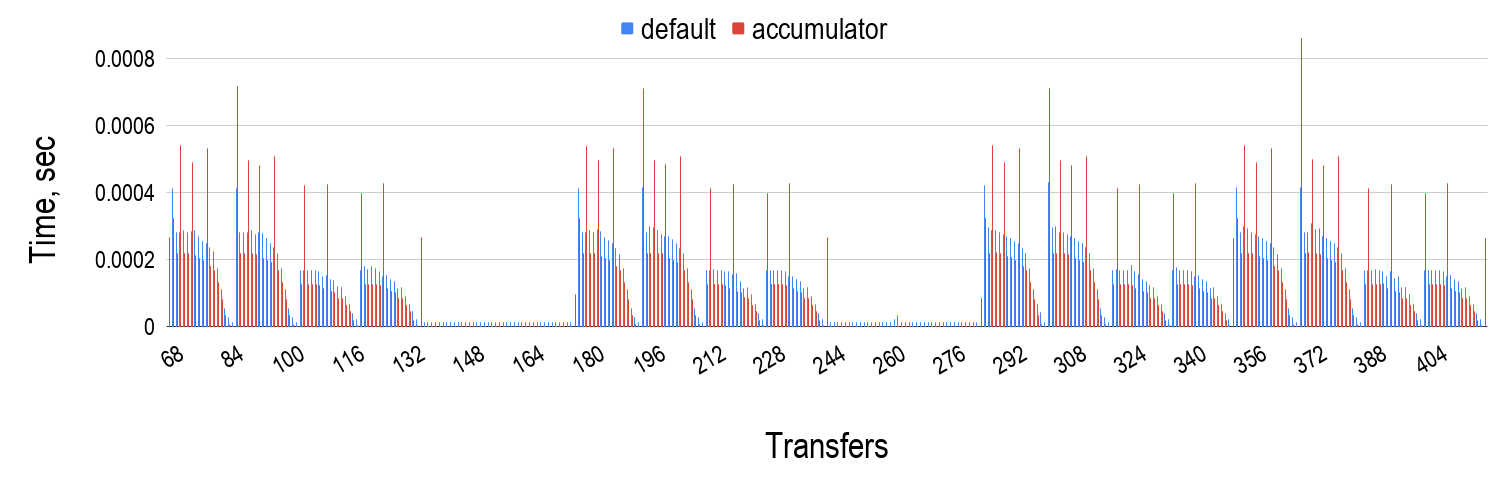
\includegraphics[width=1.0\textwidth]{figures/chapter-3/benchmark-result-non-blocking-inter-node-comm.png}
  \caption{Comparison of \textbf{BM1} benchmark with the default approach running recorded \textit{cube-64} communication pattern between two nodes}
\label{fig:benchmark:results-cube-64-inter-node-comm}
\end{figure}


The slow-down resulting from pure data accumulation could be explained by automatic \gls{mpi} protocol switching, namely: \textit{Eager} and \textit{Rendezvous} \cite{mpi:protocols-explanation}. The protocols are dedicated to small and large message transfers, respectively, where the quantitative measure of the message size is defined by a concrete implementation of the \gls{mpi} standard and can be controlled through dedicated environment variables.\\



Similar results were observed for \textit{cube-645} test case where the number of equations was approximately $10^6$ and the average compressed Jacobian column length reached around $1.7 \cdot 10^5$ elements. In case of the inter-node communication, \textbf{BM1} benchmark again showed performance degradation by \textbf{6.35\%} whereas non-blocking data broadcast improved run-time by \textbf{23.21\%}. Such performance jump, from \textbf{-6.35\%} to \textbf{23.21\%}, is explained by the fact that time spent on generation of random elements was enough to hide the corresponding data transfer and overheads.\\



Ideas, expressed in \textbf{BM1} benchmark, listings \ref{lst:bench:auxiliary-subroutines} and \ref{lst:beanch:pseudocode}, were successfully implemented in \gls{nut}: the client side of \gls{nut} located in \gls{athlet}. Several simulation scenarios were taken for the final verification and performance testing, namely: \textit{cube-64}, \textit{k3-2} and \textit{pwr3d}. Verification of the modified code did not detect any deviations of numerical results from the original implementation. Additionally, all tests showed considerable improvement with respect to the communication time. As an example, time spent on communication between \gls{athlet} and \gls{nut} during compressed Jacobian transfers decreased by \textbf{66.17\%}, \textbf{76.03\%} and \textbf{42.55\%} for intra-socket, intra-node and inter-node client-server process allocation respectively, for \textit{pwr3d} scenario, taking it as the most representative simulation case known in \gls{grs}.\\


However, the overall improvement of applied changes achieved only \textbf{0.14\%} in average, regardless of client-server allocation. Profiling showed the communication part of the original implementation took around \textbf{0.24\%} of the total time spent on the matrix evaluations and transfers. This fact explains that negligible overall performance gain of the modified code that was observed in all conducted tests.\\
